\let\negmedspace\undefined
\let\negthickspace\undefined
\documentclass[journal]{IEEEtran}
\usepackage[a5paper, margin=10mm, onecolumn]{geometry}
\usepackage{tfrupee} 
\setlength{\headheight}{1cm} 
\setlength{\headsep}{0mm}    

\usepackage{gvv-book}
\usepackage{gvv}
\usepackage{cite}
\usepackage{amsmath,amssymb,amsfonts,amsthm}
\usepackage{algorithmic}
\usepackage{graphicx}
\usepackage{textcomp}
\usepackage{xcolor}
\usepackage{txfonts}
\usepackage{listings}
\usepackage{enumitem}
\usepackage{mathtools}
\usepackage{gensymb}
\usepackage{comment}
\usepackage[breaklinks=true]{hyperref}
\usepackage{tkz-euclide} 
\usepackage{circuitikz}

\tikzstyle{block} = [rectangle, draw, fill=blue!20, 
    text width=4em, text centered, rounded corners, minimum height=3em]
\tikzstyle{sum} = [draw, fill=blue!10, circle, minimum size=1cm, node distance=1.5cm]
\tikzstyle{input} = [coordinate]
\tikzstyle{output} = [coordinate]

\begin{document}
\bibliographystyle{IEEEtran}
\vspace{3cm}

\title{MatGeo Assignment 1.2.14}
\author{AI25BTECH11008 \\ Chiruvella Harshith Sharan}

\maketitle
{\let\newpage\relax\maketitle}

\renewcommand{\thefigure}{\theenumi}
\renewcommand{\thetable}{\theenumi}
\setlength{\intextsep}{10pt}

\numberwithin{equation}{enumi}
\numberwithin{figure}{enumi}
\renewcommand{\thetable}{\theenumi}

\noindent
\textbf{Question:}\\
The fourth vertex $D$ of a parallelogram $ABCD$ whose three vertices are 
$A(-2,3)$, $B(6,7)$ and $C(8,3)$ is \\
\noindent
\textbf{Solution:}\\
We solve this using \textbf{vector algebra}.  

We are given three vertices:  
\[
A = \myvec{-2\\3}, \quad B = \myvec{6\\7}, \quad C = \myvec{8\\3}.
\]

\textbf{Property: In a parallelogram, opposite sides are parallel and equal.}  

Thus,  
\[
\vec{D} = \vec{A} + \vec{C} - \vec{B}.
\]

Substitute the values:  
\[
\vec{D} = \myvec{-2\\3} + \myvec{8\\3} - \myvec{6\\7}.
\]

\[
\vec{D} = \myvec{(-2+8-6) \\ (3+3-7)} = \myvec{0 \\ -1}.
\]

Hence,  
\[
\therefore D(0,-1)
\]

\begin{figure}[H]
    \centering
    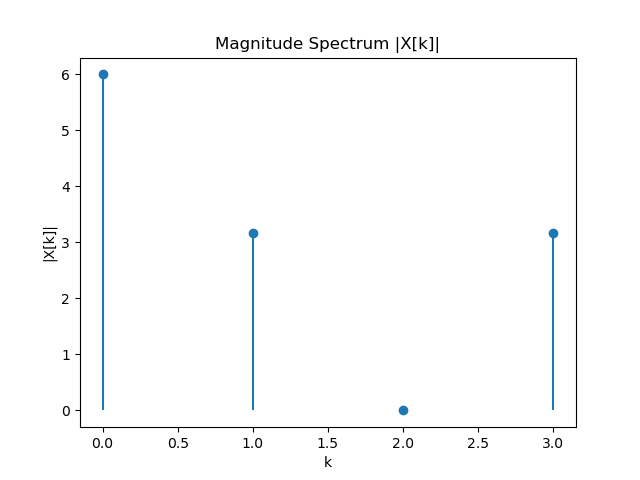
\includegraphics[width=0.75\linewidth]{figs/fig1.png}
    \caption{Parallelogram with vertices $A$, $B$, $C$, $D$ using vector method}
    \label{fig:figs/fig1.png}
\end{figure}

\noindent
Thus, using vector addition, the fourth vertex is obtained as $D(0,-1)$, which matches the computational result.

\end{document}
